\chapter{Fundamentals} % Main chapter title
\label{chap:fund}

% Hier muss alles rein was benötigt wird um die Arbeit zu verstehen.
%   Man kann ja sicherlich grundlegendes Verständis von Recherstrukturen und Organisation vorraussetzten
%   Was also sollte definitiv nochmal erklärt werden?
%
%   - Virtual Memory -> Und vor allem die Kosten, das ist ja auch irgendwo der Aufhänger
%           Der Satz, "tlb is on the critical path of everything really" sollte irgendwann mal kommen
%   - Motivation für vm
%   - Organisationsstrukturen auch im vergleich -> Fazit: Page Tables sind überall und werden tiefer -> vor allem wegeb backwards compatiblity?
%   - Hardware Strukturen für VM - MMU, TLB
%   - Operating system and VM -> Implemented by OS but fixed structures given by MMU
%   -> Problem, fehlende flexibilität ->  A look at several ...
%   -> source: Architectural and operating system support for virtual memory
%   source: issues of implementation

% -------------------------------------------------------------------------------------------------
% A little bit of history?? -> [Denning VM '96] -> Altas
% -------------------------------------------------------------------------------------------------


% -------------------------------------------------------------------------------------------------
%                                           VIRTUAL MEMORY
% -------------------------------------------------------------------------------------------------


\section{Virtual Memory}
\subsection{Motivation}
Virtual memory is used in almost every system, ranging from big data center machines to small embedded system.
Originally, it was developed by the designers of the Atlas Computer to automate the task of swaping data between
main and secondary memory \cite{denning1997before}.
This was necesarry as programs increased in size faster than main memory did; while single programs
still fit in memory, operating systems allowed running multiple programs at once, collectively exceeding
the available physical memory \cite{tanenbaumOS}.
Nowadays, virtual memory is the basis of a lot of memory system requirements such as address
space protection, isolation of processes, shared memory and more \cite{jacobSoftwaremanagedAddressTranslation1997}.
It is also completely transparent to the programmer and enables programms to use every available
address in its virtual address space.\\
Peter Denning calls its wide spread adoption ''[..]one of the engineering triumphs of the computer
age.''\cite{denning1997before}.
\subsection{Memory System Requirements/Benefits?}
% VM Properties and benefits: Was für Nutzen hat VM?
% - idealized abstraction of storage resources available on a machine
% - virtual to physical mapping
% - flexibility to place actual data anywhere on the available disk
% - emulate bigger memory than actually available
% - foundation for isolation/security
% - Implement flexible paging the swap pages between main memory and secondary storage
% Fazit: VM hat sehr nützliche Eigenschaften
% More: jacob1998virtualissues

% -------------------------------------------------------------------------------------------------
%                                IMPLEMENTATION OF VIRTUAL MEMORY
% -------------------------------------------------------------------------------------------------

% Wie können wir VM realisieren? -> Verschiedene Implementationen, Aber hier nicht auf die HW eingehen
%   [ A look at several...]
%   [ Issues of implementation]
% \section{Implementation of Virtual Memory Systems}
% \subsection{ Overview of different implementations (Inverted/Hierarchical/Multi-Level)}
% \subsection{ Comparison of differnt implementations with regards to performance and features like page sharing}
\subsection{Implementation of Virtual Memory}
Every virtual memory system has to realize a mapping from virtual addresses of each processes
private, virtual address space to actual physical addresses that index data in main memory.
This section will provide an overview of the most commonly used virtual memory implementation.

\subsubsection{Hierarchical page tables}
\begin{figure*}[t]
    \centering
    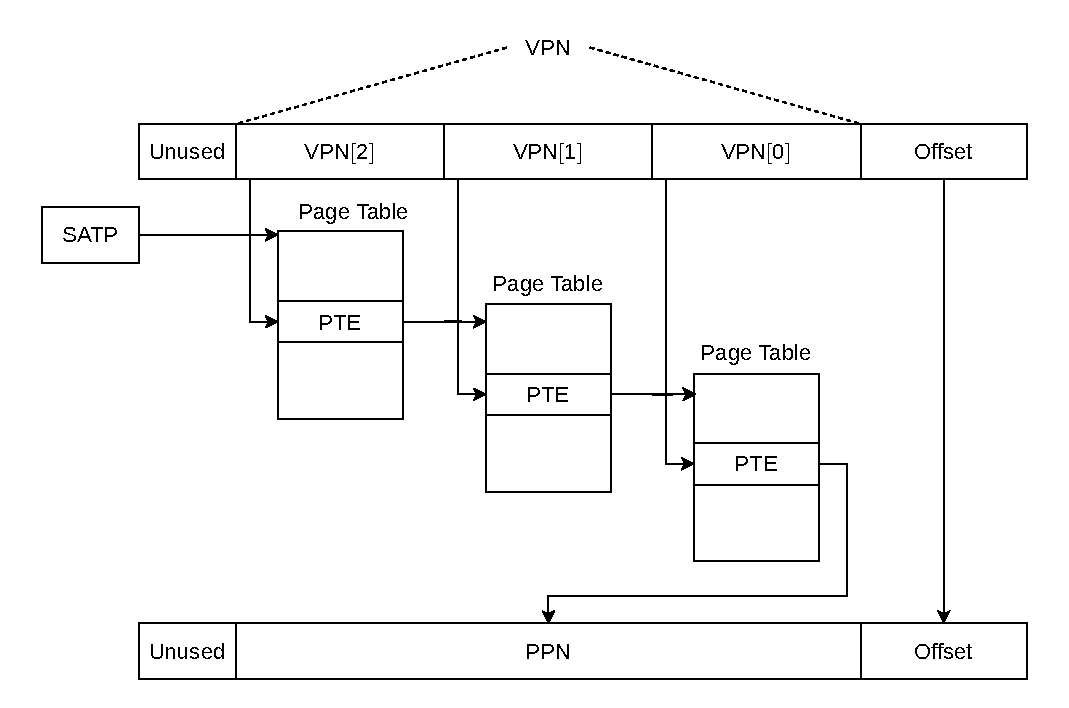
\includegraphics[scale=.8]{figures/VM-Tree.pdf}
    \caption[RISC-V Sv39 3-Level Page Tree]{Three-step page walk with a RISC-V Sv39 Page Table Tree:
        The value in the \texttt{satp} register is the base of the root page table; \texttt{VPN[2]}
        is the index into the root page table; the indexed \texttt{PTE} points to the next page table.
        This traversal continues until the bottom of the page table is reached. The last \texttt{PTE}
        contains the \texttt{PPN} of the physical address which can then be combined with the offset
        bits to make the full physical address}
    \label{fig:fund:pagetree}
\end{figure*}

% Fazit -> Viele Main Memory Zugriffe -> Teuer

% Lösung? Hashed!
\subsubsection{Inverted page tables}
\begin{figure*}[t]
    \centering
    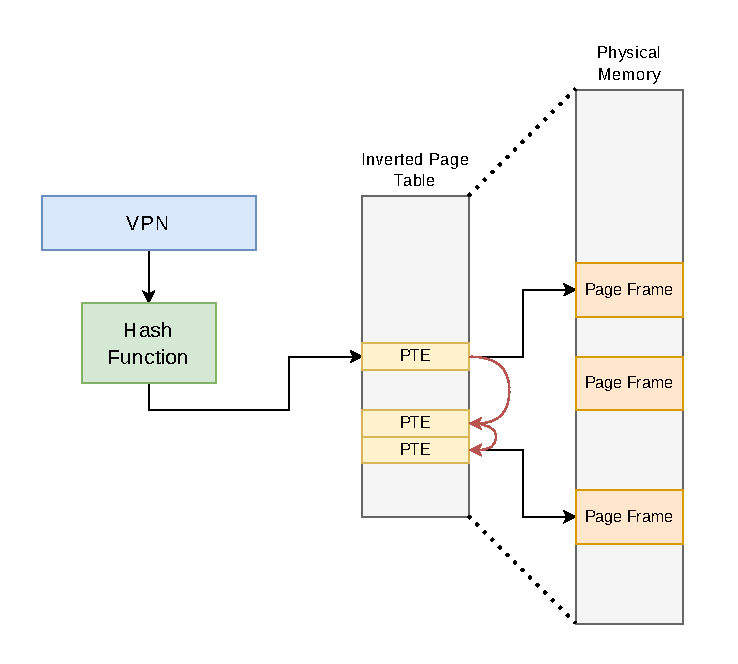
\includegraphics[scale=1]{figures/inverted_pt.pdf}
    \caption[Simple Inverted Page Table Design]{A inverted page table has an entry for every physical
        page frame, reducing memory accesses to a minimum of one. Collisions in the hash table (red arrows) can
        make the access much more expensive. }
    \label{fig:fund:pagetree}
\end{figure*}
% Fazit-> Nachteile von Invertierten Page Tables [siehe auch hash dont cache!]
% -> Most commonly used in todays hardware -> Multi level page tables
% Fazit -> Hauptproblem von VM sind teure Hauptspeicherzugriffe im kritischen Pfade von allen Memory Operations


% -------------------------------------------------------------------------------------------------
%                                  END SECTION - VM IMPLEMENTATION
% -------------------------------------------------------------------------------------------------



% -------------------------------------------------------------------------------------------------
%                                            VM HARDWARE
% -------------------------------------------------------------------------------------------------

\section{Memory Management Hardware}
\begin{figure*}[t]
    \centering
    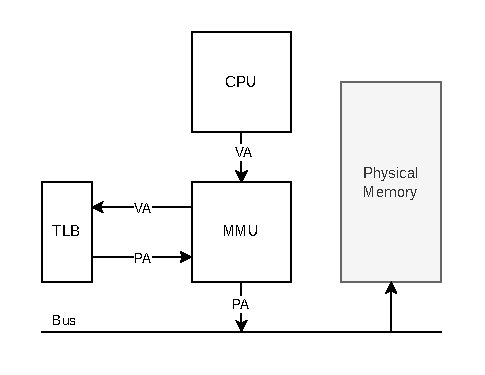
\includegraphics[scale=1.2]{figures/simple_mmu_arch.pdf}
    \caption[A simplified architecture of CPU, MMU and TLB]{A simplified architecture of CPU, MMU and TLB:
        User-level programs running on the \texttt{CPU} try to access main memory with virtual
        addresses; virtual addresses get transparently translated to physical addresses by the
        \texttt{MMU} by either looking up the address in the TLB or by performing a page table
        lookup with the hardware-supported page table design}
    \label{fig:fund:simplearch}
\end{figure*}
% Davor sollte der Page Table walk bekannt sein
\subsection{MMU}
\subsection{TLB}

% With only software ptw process would have to context switch to the kernel -> Very expensive
% With an MMU the processor essentially just freezes until the memory operation has completed
\cite{jacobVirtualMemoryContemporary1998}
% \subsection{HW-Dependent PTE Structure} -> inflexibility
% \subsection{A typical Page Table Walk}



% Fazit -> Es gibt hardware strukturen die VM beschleunigen können, die machen es auch schneller
%       ABER: Die machen die VM Software Systeme auch sehr viel rigider und unflexibler
% Kurze Diskussion -> Machen Hardware strukture das wirklich schneller? [ A look at ...]
% -------------------------------------------------------------------------------------------------

% -------------------------------------------------------------------------------------------------

\section{Sofware-based Virtual Memory System}
% VM in Software möglich mit ähnlicher Performance wie hw möglich -> Sollte ja mehr Flexibilität geben
%   [ A look at several...]
% \section{ Sofware VM Approaches}
% \section{ Liedtke GPTs}
% \subsection{More flexibilty}

\section{HW VM vs SW VM}
% related work will then come in to discuss approaches close to my approach


% -------------------------------------------------------------------------------------------------

% -------------------------------------------------------------------------------------------------

% TODO Short discussion hw and sw vm -> common problem: Page Table Walks require in either case a 
% lot of memory references. These costs can be aleviated using caches, but will still cost [ cite a source abouts costs here]

% -------------------------------------------------------------------------------------------------

% -------------------------------------------------------------------------------------------------

% All approaches are based on a table.
% Überleitung zu meinem Thema -> Avoid all memory references and just have a simple (hash?) function that realizes VM
